
\chapter{Software Implementation: \textit{CellColonySimulator}}


\begin{figure}[!htb]
    \centering


    \begin{tikzpicture}[every text node part/.style={align=center}, 
                    node distance=2cm]


    \begin{scope}[scale=0.85,transform shape]
    \node (start) [startstop] {\codeword{Master.m}};
    \node (in1) [io, below of=start] { Model parameters: $\lambda_1, ... , \lambda_7$ \\
                                       Numerical parameters: $h$, $\Delta t$ \\
                                       Run parameters: \codeword{ensembleSize}, \codeword{sampleTimes}};
    \node (pro1) [process, below of=in1] {\codeword{runSimulation.m}};
    \node (pro2) [process, below of=pro1] {\codeword{ellipse.m}};
    \node (pro3) [process, below of=pro2] {\codeword{updateFood.m}};
    \node (dec1) [decision, below of=pro3, yshift=-1.5cm] {Mitosis Condition};
    \node (pro4) [process, below of=dec1, yshift=-1.5cm] {\codeword{addCell.m}};
    \node (proNothing) [process, left of=pro4, xshift=-1.5cm] {Proceed};
    \node (pro5) [process, below of=pro4] {\codeword{updateNodes.m}};
    %\node (pro5) [process, right of=dec1, xshift=2cm] {Process 2b};
    \node (out1) [io, below of=pro5] {Run Statistics at \codeword{sampleTimes}: \\
                                      \codeword{compactness},
                                      \codeword{averageRadius},
                                      \codeword{cellCount},
                                      $\bar{\mu}$};
    \node (stop) [startstop, below of=out1] {Plot ensemble averaged results};
    \node (for) [process, left of=pro3, xshift=-3.5cm] {Loop over ensemble};
    \node (forTime) [process, right of=pro3,  xshift=3.0cm] {Loop over time};

    \draw [arrow] (start) -- (in1);
    \draw [arrow] (in1) -- (pro1);
    \draw [arrow] (pro1) -- (pro2);
    \draw [arrow] (pro2) -- (pro3);
    \draw [arrow] (pro3) -- (dec1);
    \draw [arrow] (dec1) -| node[anchor=south]{else} (proNothing);
    \draw [arrow] (proNothing) |- node[anchor=south]{} (pro5);
    \draw [arrow] (dec1) -- node[anchor=east]{if}(pro4);
    \draw [arrow] (pro4) -- (pro5);
    \draw [arrow] (pro5) -- (out1);
    \draw [arrow] (out1) -- (stop);
    \draw [arrow] (in1) -| node[anchor=south]{} (for);
    \draw [arrow] (for)  |- node[anchor=south]{} (out1);
    \draw [arrow] (pro1)  -| node[anchor=south]{} (forTime);
    \draw [arrow] (forTime)  |- node[anchor=south]{} (pro5);
    
    %\draw [arrow] (pro2a) -- (out1);
    %\draw [arrow] (out1) -- (stop);

    \end{scope}
\end{tikzpicture}
\caption{A flow chart of \textbf{CellColonySimulator} software package in MATLAB. }
\label{fig:softwareFlowChart}
\end{figure}

\section{The structure of the program}
The program \textbf{CellColonySimulator} is implemented \textit{in-house} with MATLAB as shown in 
figure \ref{fig:softwareFlowChart}. \textbf{CellColonySimulator} is broken up 
into six seperate scripts as per the programming principle of modularity. These include:
\codeword{Master.m},
\codeword{runSimulation.m},
\codeword{ellipse.m},
\codeword{updateFood.m},
\codeword{addCell.m},
\codeword{updateNodes.m}.

\subsection{Calling the update loop in \textit{runSimulation.m}}\label{ssec:runSimulation}
The function \codeword{runSimulation.m} takes in the model parameter vector,
$\lambda$, the struct of numerical discretisation parameters, \codeword{numericPack},
the times at which statistics are sampled, \codeword{sampleTimes}, 
the colony data including node positions $(x,y)$ and the network adjacency
matrix, \codeword{connectivity}, and the initial nutrient field 
given by \codeword{food}.
\\

The mesh grid matrices $X$ and $Y$ are taken from \codeword{numericPack} and 
converted to graphics processing unit (GPU) arrays using MATLAB's \codeword{gpuArray()}. This is crucial 
for speed as GPU operations on large matrices are highly optimised and parallelised within 
the GPU architecture. Besides generating descriptive file names for the output plots
and other miscellaneous tasks, \codeword{runSimulation.m} then progresses into 
the primary \codeword{for} loop over the time indices, \codeword{timeIndex}.
\\

A task to print to the console to let the user know what ensemble instance
and \codeword{timeIndex} the program is up to, is done first.
Secondly, based on the current node positions $(x_i,y_i)$ for
$i \in \{1, ..., N_{\textrm{nodes}}\}$, and the number
of edges present in the \codeword{connectivity} matrix, the current number of cells
$N_{\textrm{cells}}$ is counted up
and vectors are associated to the variables $x_{c,k}$,$y_{c,k}$,
$\theta_k$, $p_k$ and $q_k$ (based on equations
 \ref{eqn:semiMajorAxis}, \ref{eqn:semiMinorAxis},
\ref{eqn:orientationAngle} and \ref{eqn:centerPos}) where $k \in \{1, ..., N_{\textrm{cells}}\}$.
These vectors are passed to the function \codeword{ellipse()} (explained in 
subsection \ref{ssec:ellipse})
which computes the colony-level signed distance field (SDF),
which is comprised of the elliptical SDF of each cell indexed $k$.
\\

At this stage the biomass field, \codeword{biomass}, is computed 
from the colony level SDF, based on equation \ref{eqn:biomass}.
The current value of the nutrient field and the biomass field,
are passed to \codeword{updateFood()} (explained in 
subsection \ref{ssec:updateFood}) which updates the nutrient field
based on the Crank-Nicholson method applied to equation \ref{eqn:EOMs_PDE}.
The food at the next time step is the output from \codeword{updateFood()}.
\\

The value of the growth rate across the colony $\mu_i$ is then determined
using 2D interpolation by calling \codeword{interp2(X, Y, food, x, y)},
where $X, Y$ are the underlying grid matrices, \codeword{food} is the updated nutrient 
field, and $(x,y)$ are the node positions, taken as query points in the interpolation.
Recall from equation \ref{eqn:growthRate}, the growth rate 
is given by the the average of the nutrient field sampled over the nodes.
\\

The updated number of nodes, $N_{\textrm{nodes}}' = N_{\textrm{nodes}}(t_{n + \Delta n})$, is found 
by multiplying the current number of nodes, $N_{\textrm{nodes}}$,
by $e^{\mu}$ (as stipulated by the exponential growth in equation \ref{eqn:expGrowth}) where $\mu$ is the average growth rate over the colony 
as discussed above. The number of nodes added is then given by 
\begin{equation*}
    \Delta N_{\textrm{nodes}} = N_{\textrm{nodes}}' - N_{\textrm{nodes}} = \lceil e^{\mu} -1 \rceil N_{\textrm{nodes}},
\end{equation*}
where $\mu$ is given by 
\begin{equation*}
    \mu = \frac{1}{N_{\textrm{nodes}}} \sum_{i = 1}^{N_{\textrm{nodes}}} \mu_i,
\end{equation*}
where $\mu_i = c(\vb{x}_i, t)$ is the value of the nutrient field $c(\vb{x}_i, t)$ sampled 
at the $i$-th node position (this is just a recapitulation of equation \ref{eqn:growthRate}).
The number of time steps per mitosis event, $\Delta n$ is given by \codeword{ceil(1.0/dt)},
and we use an \codeword{if} statement to ensure \codeword{addCell()} is only called when $n$ 
is a multiple of $\Delta n$.
\\

In \codeword{addCell()}, the number of nodes to add, $\Delta N_{\textrm{nodes}}$, is passed 
as a argument. The mechanism to choose the parent cells to undergo mitosis is 
explained in subsection \ref{ssec:addCell}. Finally, 
the new node positions (based on equation \ref{eqn:EOMs_ODE}) are determined 
using \codeword{updateNodes()} as detailed in subsection \ref{ssec:updatenodes}.
\\

The rest of \codeword{runSimulation.m} is devoted to plotting the biomass and nutrient 
fields, aswell as generating the underlying node network using MATLAB's 
\codeword{graph()} where the colony adjacency matrix, \codeword{connectivity},
is passed as an argument.


\subsection{Vectorised computation of colony SDF in \textit{ellipse.m}}\label{ssec:ellipse}
The custom function \codeword{ellipse.m} has been iterated
with high efficiency in mind since \codeword{ellipse.m} has to be called 
every time step. Using MATLAB's widget \textit{run-and-time}, the bottleneck found
in \codeword{ellipse.m} was eliminated. This significantly 
improved run times. How was this speedup achieved?
\\

Where previously \codeword{ellipse.m} required a \codeword{for} loop over the SDFs for 
each cell, the final iteration of \codeword{ellipse.m} uses 
completely vectorised operations which run fast on the GPU. The code is 
provided in listing \ref{lst:ellipse}.

\begin{lstlisting}[style=Matlab-editor,  
                   caption={A code listing for the \textbf{ellipse.m} script},
                   label={lst:ellipse}]
function sdf =                ... %Colony level SDF
    ellipse(X, Y,             ... %Grid values
            theta,            ... %Orientation angles
            centerX, centerY, ... %Center coordinates
            semiMajorRadius,  ... %p_k
            semiMinorRadius   ... %q_k       
           ) 
    %Translate the field to the center coordinates:
    Xt = repmat(X, [1,1,size(centerX,2)])-reshape(centerX, [1,1,size(centerX,2)]);
    Yt = repmat(Y, [1,1,size(centerX,2)])-reshape(centerY, [1,1,size(centerX,2)]);
    %Precompute trigonometric functions for efficiency
    COS = cos(theta);
    SIN = sin(theta);
    cosReshape = reshape(COS, [1,1,size(centerY,2)]);
    sinReshape = reshape(SIN, [1,1,size(centerY,2)]);
    %Rotate translated field by the rotation matrix (correctly vectorised):
    rotX =  Xt .* cosReshape + Yt .* sinReshape; 
    rotY = -Xt .* sinReshape + Yt .* cosReshape;
    %Precompute reciprocal squared of geometry arrays:
    semiMajorRadiusReciprocalReshape2 = ... 
        reshape(1.0 ./ semiMajorRadius.^2, [1,1,size(centerX,2)]);
    semiMinorRadiusReciprocalReshape2 = ...
        reshape(1.0 ./ semiMinorRadius.^2, [1,1,size(centerX,2)]);
    %Instead of using smoothmin (slow) just use min of the
    %square of the SDF. [This does not require calling sqrt() 
    %which is computationally very costly]
    sdf = min(rotX .^2 .* semiMajorRadiusReciprocalReshape2 + ...
              rotY .^2 .* semiMinorRadiusReciprocalReshape2 - ... 
              1.0, [], 3);
    %Normalise to with magnitude 1 in colony region:
    absMin = abs(min(sdf,[], "all"));
    sdf = sdf ./ absMin ;
end    
\end{lstlisting}

One thing to note from the MATLAB code listing is that 
vectorised division, say called with \codeword{./}, 
is precomputed as reciprocals which 
are then multiplied through in the compuatation of \codeword{sdf} using \codeword{.*} which is 
faster. Precomputing trigonometric functions was also opted for with 
the aim of reducing repeated compuatations with the same angle. 
Finally, we recall the discussion in section \ref{sec:introSDFs}, in which 
it was noted that \codeword{min} is significantly faster than evaluating smoothmin. 
The final optimisation made was to remove the call to \codeword{sqrt()} which  
actually has no effect on the shape of each cell but vastly improves
compute time.


\subsection{A fast Crank-Nicolson scheme in \textit{updateFood.m}}\label{ssec:updateFood}
The Crank-Nicolson scheme is an implicit numerical scheme that requires the 
computation of a (mostly zero) matrix of coefficients \codeword{LHM} (which has 
dimensions $N_{\textrm{grid}}^2 \times N_{\textrm{grid}}^2$)
a right hand side column vector \codeword{RHS} ($N_{\textrm{grid}}^2 \times 1$), and the 
solution of the linear system 
\codeword{LHM * x = RHS}. 
\\

The most obvious optimisation made in \codeword{updateFood()} 
is to completely vectorise all operations. As evinced in the code given in 
listing \ref{lst:updateFood}, there are no \codeword{for} loops.

\begin{lstlisting}[style=Matlab-editor,basicstyle=\lstconsolas,basicstyle=\small,  
                   caption={A code listing for the \textbf{updateFood.m} script. The variable
                   name \textbf{CFL} refers to the Courant–Friedrichs–Lewy number 
                   which comes up in numerical schemes. This is called $\alpha$ in 
                   Chapter 1.},
                   label={lst:updateFood}]
function foodNew = updateFood(biomass, food, lambda, dt, h, X)
    N = size(X,1);
    V = N .* N;
    Vi = (N-2) .* (N-2);
    i = 2:(N-1);
    j = i;  
    %Generate the five point stencil of indices in row major order.
    ij   = rmo(i,j,N);
    im1j = rmo(i-1,j,N);
    ip1j = rmo(i+1,j,N);
    ijm1 = rmo(i,j-1,N);
    ijp1 = rmo(i,j+1,N);
    %Flatten these:
    fij   = ij(:);
    fim1j = im1j(:);
    fip1j = ip1j(:);
    fijm1 = ijm1(:);
    fijp1 = ijp1(:);

    CFL = dt .* lambda(1) ./ (h .* h);
    coeff1 = 0.5 .* dt .* biomass(i,j) + 2.0 .* CFL + 1.0;
    coeff2 = 0.5 .* CFL;
    coeff3 = 1.0 - 2.0 .* CFL - 0.5 .* dt .* biomass(i,j);
    %Flatten the coefficients:
    coeff1 = coeff1(:);
    coeff3 = coeff3(:);
    c = food(:);

    RHS = coeff3 .* c(fij) + ...
          coeff2 .* (c(fim1j) + c(fip1j) + c(fijm1) + c(fijp1));

    LHM = spdiags([-coeff2 .* ones(Vi,1) ,-coeff2 .* ones(Vi,1) ,...
                   gather(coeff1),...
                   -coeff2 .* ones(Vi,1), -coeff2 .* ones(Vi,1)],...
                  [-N, -1, 0, 1, N], Vi, Vi);
    yM  = spdiags(-coeff2 .* ones(1,N), 0, N, N);
    LHM(1:N,(end - N + 1):end) = LHM(1:N,(end - N + 1):end) + yM;
    LHM((end - N + 1):end,1:N) = LHM((end - N + 1):end,1:N) + yM;

    [cNew, flag] = pcg(LHM,RHS,1e-6);

    foodNew = food;

    foodNew(i,j) = reshape(cNew, [N-2, N-2]);
end


function index = rmo(i,j,N)
    index = i' + N .* (j-1);
end
\end{lstlisting}

Another optimisation which was not only efficient but also necessary to avoid
memory issues, was to construct \codeword{LHM} with sparse matrices, which 
meant that on the order of $N_{\textrm{grid}}^4$ redundant zeros did not have 
to be stored in memory. In particular, the pentadiagonal matrix ($5$ non-zero diagonals)
 \codeword{LHM} was constructed using \codeword{spdiags}. A crucial optimisation 
from the point of view of perfomance was to 
replace the direct linear solution, \codeword{LMH \ RHS}, with the function, 
\codeword{pcg}, which carries out the preconditioned conjugate 
gradient numerical method at no appreciable change in accuracy (error bounded by \codeword{1e-6}),
but significantly faster.
\\

Regarding indexing, note that MATLAB uses column-major-order by default in 
its vectorised functions (see MathWorks website). To align with this convention,
the row-major-order function, \codeword{rmo}, transposes the row indices, \codeword{i},
and leaves the column indices, \codeword{j}, fixed. Other configurations were 
trialed but this was ultimately the only one that produced the correct 
nutrient diffusion dynamics.

\subsection{Introducing new nodes in \textit{addCell.m}} \label{ssec:addCell}
Adding in $\Delta N_{\textrm{nodes}}$ new nodes to the colony requires the
selection of $\Delta N_{\textrm{nodes}}$ parent nodes to undergo 
mitosis. This is choice is based on first interpolating the nutrient 
available to each node, and using \codeword{maxk()} to decide on the 
$\Delta N_{\textrm{nodes}}$ parent node indices corresponding to 
greatest values of \codeword{food}. These are called 
\codeword{buddingIndices} in the \codeword{addCell.m} script. 
The new node positions are defined by first generating a random 
budding angle, $\theta_b$, for each node to be added. The formula for 
a child node's position is given by 
\begin{equation*}
x_{\textrm{child}} = x_{\textrm{parent}} + \delta \cos{\theta_b},
\end{equation*}
\begin{equation*}
y_{\textrm{child}} = y_{\textrm{parent}} + \delta \sin{\theta_b},
\end{equation*}
where $\delta = 0.01$ is a very small dislocation radius.
\\

Finally, the addition of new nodes implies the addition of new cells which 
are defined by the edge connecting a pair of nodes. This 
change in the adjacency matrix requires updating the \codeword{connectivity}
array by placing a $1$ in the correct positions. Recall that 
the \codeword{connectivity} array is a symmetric logical matrix.

\subsection{Advancing the node positions using Euler's method in \textit{updateNodes.m}} \label{ssec:updatenodes}
The \codeword{updateNodes.m} script employs Euler's first order
time marching algorithm to update the node positions, 
based on three forces: elasticity, contact and chemotaxis. 
It was conceivable that a Runge-Kutta-$4$ (RK4) explcit time stepping scheme,
 detailed in \cite{zingg1999runge},
could have been implemented, however this was deemed to be unnecessary since
determining the overdamped spring dynamics to a high degree of accuracy 
is always swamped by the overall conceptual errors in the modelling. 
From a mathematical modelling point of view, the spring has been 
chosen to ensure the passage of the colony from one equilibrium state 
at the old number of nodes, $N_{\textrm{nodes}}$, to the equilibrium state 
at the updated node count, $N_{\textrm{nodes}}'$. The Euler method 
was sufficient to allow this transition without 
any numerical stability issues. The code is given  in listing \ref{lst:updateNodes}.

\begin{lstlisting}[style=Matlab-editor,basicstyle=\lstconsolas,basicstyle=\small,  
                   caption={A code listing for the \textbf{updateNodes.m} script},
                   label={lst:updateNodes}]
function [xNew,yNew] = updateNodes(x, y, lambda, connectivity, food, numNodes, dt, h, X,Y)
    %Firsly calculuate the matrix of distances between the nodes;
    xNodes = x(1:numNodes);
    yNodes = y(1:numNodes);
    xMatrix = gpuArray(xNodes - xNodes');
    yMatrix = gpuArray(yNodes - yNodes');
    matrixOfSquares = xMatrix.^2 +  yMatrix.^2;
    matrixOfSquaresDivisor = matrixOfSquares + (matrixOfSquares == 0);
    rSQRT = 1 ./ sqrt(matrixOfSquaresDivisor);

    xNew = x;
    yNew = y;
    contactMask = double(matrixOfSquares <= lambda(4).^2); 
    connectivityNodes = double(connectivity(1:numNodes,1:numNodes ));

    %Add the force due to the spring:
    springTermX = (1.0 - rSQRT) .* xMatrix;
    springTermX = springTermX .* connectivityNodes;
    springTermY = (1.0 - rSQRT) .* yMatrix;
    springTermY = springTermY .* connectivityNodes;

    xNew(1:numNodes) = xNew(1:numNodes) - ...
    dt .* lambda(2) .* sum(springTermX, 2);   
    yNew(1:numNodes) = yNew(1:numNodes) - ...
    dt .* lambda(3) .* sum(springTermY, 2);

    contactTermX =  rSQRT .* xMatrix;
    contactTermX = contactTermX .* contactMask;
    contactTermY =  rSQRT .* yMatrix;
    contactTermY = contactTermY .* contactMask;
    
    %Add in the contact force:
    xNew(1:numNodes) = xNew(1:numNodes) + ...
       dt .* lambda(1) .* sum(contactTermX, 2);
    yNew(1:numNodes) = yNew(1:numNodes) + ...
       dt .* lambda(1) .* sum(contactTermY, 2);

    [foodGradientX, foodGradientY] = gradient(food,h);

    %Sample the gradient at the nodes:
    foodGradientXAtNodes = interp2(X,Y,foodGradientX, xNodes,  yNodes );
    foodGradientYAtNodes = interp2(X,Y,foodGradientY, xNodes,  yNodes );

    %Add in the chemotactic force:
    xNew(1:numNodes) = xNew(1:numNodes) +  dt .* lambda(5) .* foodGradientXAtNodes;
    yNew(1:numNodes) = yNew(1:numNodes) +  dt .* lambda(5) .* foodGradientYAtNodes;
end
\end{lstlisting}
Note that the \codeword{matrixOfSquaresDivisor} is constructed in such a way 
as to avoid introducing \codeword{nan} values into the solution.


\section{Statistics from the model}
The software developed thus far is a numerical framework for simulating growing cell colonies.
There is an element of randomness in the model: when two nodes are dislodged from the 
same point there is initially no preferred direction to move in so one must be chosen randomly
before other forces can take effect. For this reason, every seperate run of the model 
starting with identical initial conditions will look different after some time. 
It is expected, however, that some ``averaged''
quantity will stabilise so long as the model is simulated over a fairly large number of runs.
Seperate runs of the model belong to a set called an ensemble.
\\

A fully grown colony will in general not be perfectly circular in shape.
In order to measure the roundness of the colony (or analagously, the degree of branching) 
we use the compactness metric used for 
 roundness in image processing (for example, see \cite{li2024off}). This is given by
\begin{equation}
  C = \frac{P^2}{4 \pi A},
\end{equation}
where $C \in [1, \infty)$ is $1$ for a circle and can get to large numbers for 
highly branching shapes, $A$ is the colony area, and $P$ is the colony perimeter. 
Both of these are calculated from the colony SDF changes sign. 
\\

A black and white image 
is produced at each time step using Matlab's function \codeword{bwboundaries} as per
PhD student Kai Li's implementation. The area then is given by summing up the grid squares that are
inside the implicit shape given by the SDF and multiplying by $h^2$. The perimeter
is obtained by using \codeword{bwboundaries}, which outputs an array of points on the boundary
from which the Euclidean distance between neighbouring points is found and then summed over.
Figure \ref{fig:compactness_comparison} demonstrates visually that more branched shapes 
have higher compactness than approximately circular shapes.
\begin{figure}[!htb]
    \centering
    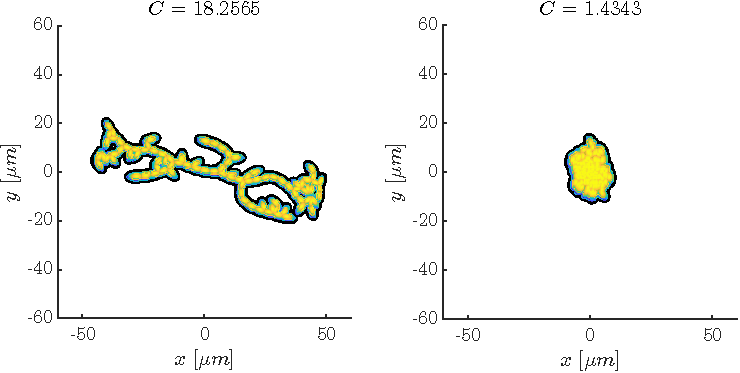
\includegraphics[width=\textwidth]{chapter1/figures/compareCompactness.pdf}
    \caption{A comparsion of high and low compactness}
    \label{fig:compactness_comparison}
\end{figure}
The summary statistics descriptions are collected in table \ref{table:summaryStats}.
\begin{table}[!htb]
\begin{center}
    \begin{tabular}{ |c|c|c| } 
     \hline
      \textbf{Symbol} & \textbf{Description} \\ 
      \hline
     $C$                 &  Colony compactness. \\ 
     $\mu$               & Colony average growth rate. \\ 
     $\bar{d}$           &   Average distance of cells from origin. \\ 
     $N_{\textrm{cells}}$ & Cell count. \\
     \hline   
    \end{tabular}   
\end{center}
\caption{The summary statistics extracted from the model}
\label{table:summaryStats}
\end{table}












